% Created 2016-01-16 Sat 12:26
\documentclass[11pt]{article}
\usepackage[utf8]{inputenc}
\usepackage[T1]{fontenc}
\usepackage{fixltx2e}
\usepackage{graphicx}
\usepackage{longtable}
\usepackage{float}
\usepackage{wrapfig}
\usepackage{rotating}
\usepackage[normalem]{ulem}
\usepackage{amsmath}
\usepackage{textcomp}
\usepackage{marvosym}
\usepackage{wasysym}
\usepackage{amssymb}
\usepackage{hyperref}
\tolerance=1000
\usepackage[utf8]{inputenc}
\usepackage{commath}
\usepackage{pgf}
\usepackage{tikz}
\usetikzlibrary{shapes,backgrounds}
\usepackage{marginnote}
\usepackage{listings}
\usepackage{enumerate}
\usepackage{algpseudocode}
\usepackage{algorithm}
\usepackage{mathtools}
\usetikzlibrary{arrows,automata}
\setlength{\parskip}{16pt plus 2pt minus 2pt}
\renewcommand{\arraystretch}{1.6}
\DeclareMathOperator{\Neg}{Neg}
\author{Oleg Sivokon}
\date{\textit{<2016-01-01 Fri>}}
\title{Assignment 15, Authomata Theory}
\hypersetup{
  pdfkeywords={Automata Theory, Formal Languages, Assignment},
  pdfsubject={Fifth assignment in the course 20440 Automata and Formal Languages},
  pdfcreator={Emacs 24.5.1 (Org mode 8.2.10)}}
\begin{document}

\maketitle
\tableofcontents


\definecolor{codebg}{rgb}{0.96,0.99,0.8}
\definecolor{codestr}{rgb}{0.46,0.09,0.2}
\lstset{%
  backgroundcolor=\color{codebg},
  basicstyle=\ttfamily\scriptsize,
  breakatwhitespace=false,
  breaklines=false,
  captionpos=b,
  framexleftmargin=10pt,
  xleftmargin=10pt,
  framerule=0pt,
  frame=tb,
  keepspaces=true,
  keywordstyle=\color{blue},
  showspaces=false,
  showstringspaces=false,
  showtabs=false,
  stringstyle=\color{codestr},
  tabsize=2
}
\lstnewenvironment{maxima}{%
  \lstset{%
    backgroundcolor=\color{codebg},
    escapeinside={(*@}{@*)},
    aboveskip=20pt,
    captionpos=b,
    label=,
    caption=,
    showstringspaces=false,
    frame=single,
    framerule=0pt,
    basicstyle=\ttfamily\scriptsize,
    columns=fixed}}{}
}
\makeatletter
\newcommand{\verbatimfont}[1]{\renewcommand{\verbatim@font}{\ttfamily#1}}
\makeatother
\verbatimfont{\small}%
\clearpage

\section{Problems}
\label{sec-1}

\subsection{Problem 1}
\label{sec-1-1}
Given context-free grammar $V = \{S,M,N,W,X,Y,Z\}$ s.t. $T=\{1,0\}$

\begin{align*}
  &S \to M \;|\; XN \;|\; W \;|\; 0N \;|\; 1Z1 \\
  &M \to 0M0 \;|\; N \\
  &N \to N0 \;|\; 0 \\
  &W \to 0W \;|\; 00W0 \\
  &X \to 0X1 \;|\; 0 \;|\; 0Y0 \\
  &Z \to W \;.
\end{align*}


\begin{enumerate}
\item Is $V$ ambiguous?
\item Give a normalized grammar equivalent to $V$.
\end{enumerate}

\subsubsection{Answer 2}
\label{sec-1-1-1}
It is easier to normalize the grammar first and then to look for ambiguities,
thus the answers are in reverse order.
\begin{enumerate}
\item Any derivation containing $W$ cannot terminate, and so does $Z$.
\item Further, we can eliminate the rule $M \to N$.
\item $Y$ has no derivation rules, thus we can also remove it.
\end{enumerate}

Thus obtaining:
\begin{align*}
  &S \to M \;|\; XM \;|\; 0M \\
  &M \to 0M0 \;|\; 0 \;|\; 0M \\
  &X \to 0X1 \;|\; 0 \;.
\end{align*}

\begin{enumerate}
\item It is easy to see that $M$ derives number of zeros greater than one,
thus $M \to 0M0$ is redundant.  Subsequently, $S \to 0M$ is already
covered by $S \to M$.
\end{enumerate}


What remains is:
\begin{align*}
  &S \to M \;|\; XM \\
  &M \to 0 \;|\; 0M \\
  &X \to 0 \;|\; 0X1 \;.
\end{align*}

\subsubsection{Answer 1}
\label{sec-1-1-2}
Now it is easy to see that the string 00 can be derived in two different
ways:

\begin{itemize}
\item $S \to M$, $M \to 0M$, $M \to 0$.
\item $S \to XM$, $X \to 0$, $M \to 0$.
\end{itemize}

Hence $V$ is ambiguous.
\subsection{Problem 2}
\label{sec-1-2}
Given context-free grammar $V = \{S,M,N,W,X,Y,Z\}$ s.t. $T=\{1,0\}$

\begin{align*}
  &S \to 0W11 \;|\; 0X1 \;|\; 0Y \\
  &W \to S \;|\; Z \\
  &X \to S \;|\; W \\
  &Y \to 1 \\
  &Z \to X \;.
\end{align*}


\begin{enumerate}
\item Bring $V$ to Chomsky's normal form.
\item What is the language of $V$?
\end{enumerate}

\subsubsection{Answer 3}
\label{sec-1-2-1}
\begin{enumerate}
\item We can easily eliminate $Y$ variable, thus removing $Y \to 1$ rule,
and adding $S \to 01$ rule.
\item We can eliminate $Z$ variable by removing $Z \to X$ and $W \to Z$ rules
and adding $W \to X$ rule.
\item We can eliminate $X$ variable by removing $X \to S \;|\; W$ and $S \to
       0X1$ rules, and adding: $S \to 0S1$ rule.
\item Finally, we can eliminate $W$ variable by removing $W \to S$ and $S \to
       0W11$ rules and adding $S \to 0S11$ rule.
\end{enumerate}


The resulting grammar will be:

\begin{align*}
  &S \to 0S11 \;|\; 0S1 \;|\; 01 \;.
\end{align*}


Since this is still not CNF, I introduce an extra variable: $X$ and
derivation rules $X \to 0$, $Y \to 1 \;|\; 11$ and $Z \to SY$ thus
obtaining:

\begin{align*}
  &S \to XZ \;|\; 01 \\
  &X \to 0 \\
  &Y \to 1 \;|\; 11 \\
  &Z \to SY \;.
\end{align*}


Which is in CNF.

\subsubsection{Answer 4}
\label{sec-1-2-2}
Using the results from the previous answer it is easy to see that
the language $L(V)=\{0^n1^k \;|\; n \leq k \land n,k > 0\}$.

\subsection{Problem 3}
\label{sec-1-3}
Build a PDA accepting the language $L$ by emptying the stack.

\begin{align*}
  L = \{ a^{i_1}b^{j_1}a^{i_2}b^{j_2}\dots a^{i_m}b^{j_m}
       &\;|\; m \geq 1 \\
       &\;|\; \forall k: i_k \geq j_k \geq 1 \\
       &\;|\; \exists k: i_k > j_k \}
\end{align*}

\subsubsection{Answer 5}
\label{sec-1-3-1}
First, I'll write the grammar for $L$ (because it's easier to do):

\begin{align*}
  &S \to aSb \;|\; K \;|\; SS \\
  &K \to aKb \;|\; aaXb \\
  &X \to aXb \;|\; aaXb \;|\; \epsilon \;.
\end{align*}

\begin{enumerate}
\item $X$ generates strings of the form $\{ a^nb^m \;|\; n \geq m \}$.
\item Similarly, $K$ generates strings of the form $\{ a^nb^m \;|\; n > m \}$.
\item The derivatin of $S$ can only terminate when it eventually derives $K$.
It can repeat as many times as needed to accept the entire string.  Where
the repeated element is, again, of the form of either $\{ a^nb^m \;|\; n
       \geq m \}$, or $\{ a^nb^m \;|\; n > m \}$.
\end{enumerate}

Thus, at least informally, we are convinced the grammar generates $L$.

Now, the automaton:

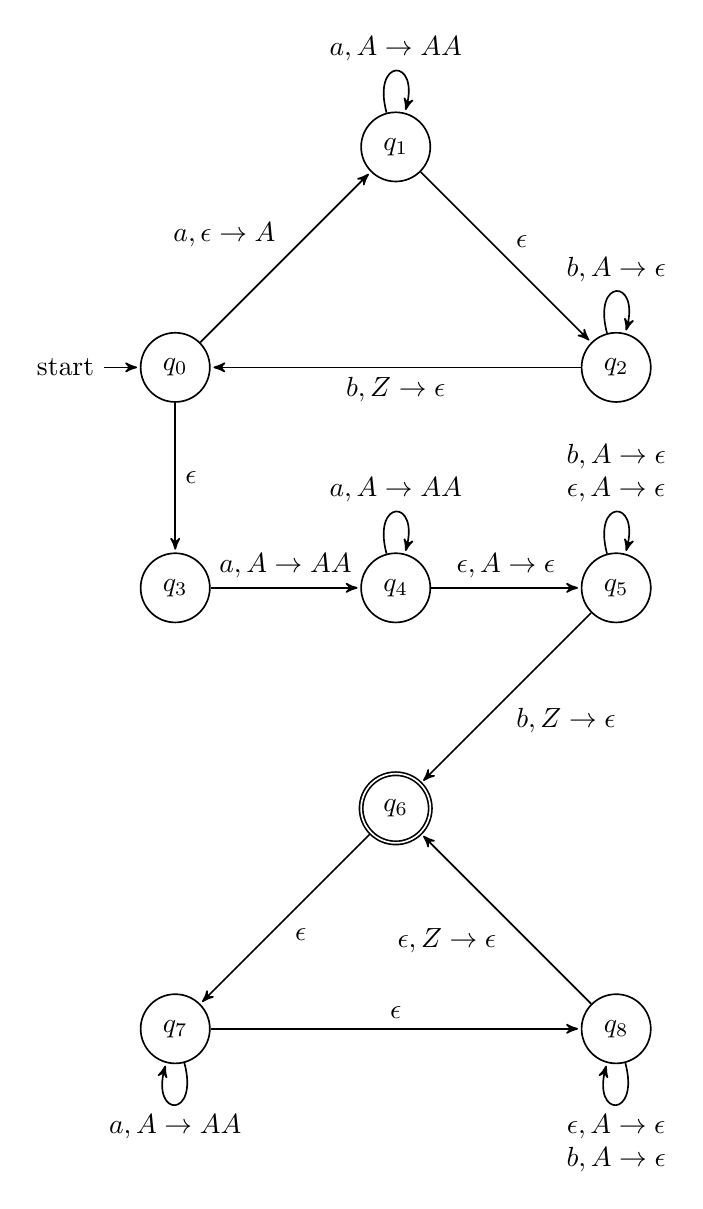
\begin{tikzpicture}[->,>=stealth',shorten >=1pt,auto,node distance=2.8cm,
                    semithick]

  \node[initial,state]   (A)                          {$q_0$};
  \node[state]           (B) [right of=A, above of=A] {$q_1$};
  \node[state]           (C) [right of=B, below of=B] {$q_2$};
  \node[state]           (D) [below of=A]             {$q_3$};
  \node[state]           (E) [right of=D]             {$q_4$};
  \node[state]           (F) [right of=E]             {$q_5$};
  \node[accepting,state] (G) [below of=E]             {$q_6$};
  \node[state]           (H) [left of=G, below of=G]  {$q_7$};
  \node[state]           (J) [right of=G, below of=G] {$q_8$};

  \path (A) edge              node {$a, \epsilon \to A$}         (B)
            edge              node {$\epsilon$}                  (D)
        (B) edge [loop above] node {$a, A \to AA$}               (B)
            edge              node {$\epsilon$}                  (C)
        (C) edge [loop above] node {$b, A \to \epsilon$}         (C)
            edge              node {$b, Z \to \epsilon$}         (A)
        (D) edge              node {$a, A \to AA$}               (E)
        (E) edge [loop above] node {$a, A \to AA$}               (E)
            edge              node {$\epsilon, A \to \epsilon$}  (F)
        (F) edge [loop above, align=center] node {
                                    $b, A \to \epsilon$ \\
                                    $\epsilon, A \to \epsilon$}  (F)
            edge              node {$b, Z \to \epsilon$}         (G)
        (G) edge              node {$\epsilon$}                  (H)
        (H) edge [loop below] node {$a, A \to AA$}               (G)
            edge              node {$\epsilon$}                  (J)
        (J) edge [loop below, align=center] node {
                                    $\epsilon, A \to \epsilon$ \\
                                    $b, A \to \epsilon$}         (J)
            edge              node {$\epsilon, Z \to \epsilon$}  (G);
\end{tikzpicture}

The idea behind this diagram is as follows:
\begin{enumerate}
\item Loop as many times as needed (possibly zero) over strings $a^nb^n$, where
$n \geq 1$.
\item Nondeterministically parse a string $a^nb^m$ where $n > m$.
\item Loop as many times as needed (possibly zero) over strings $a^nb^m$ where
$n \geq m$.
\item Before accepting state, keep discarding $A$ until none remain for as long as
you don't see an $a$.
\item Accept the string.
\end{enumerate}

\subsection{Problem 4}
\label{sec-1-4}
Construct a PDA for $L$ defined as follows:
\begin{align*}
  L = \{ dw_1dw_2d\dots w_nd
       &\;|\; n \geq 3 \\
       &\;|\; \forall k: w_k \in \{a,b,c\}^* \\
       &\;|\; \exists k: 1 \leq k \leq n - 2 \land \abs{w_k} = \#_c(w_{k+2}) \}
\end{align*}

\subsubsection{Answer 6}
\label{sec-1-4-1}
The automaton for $L$ may look like this:

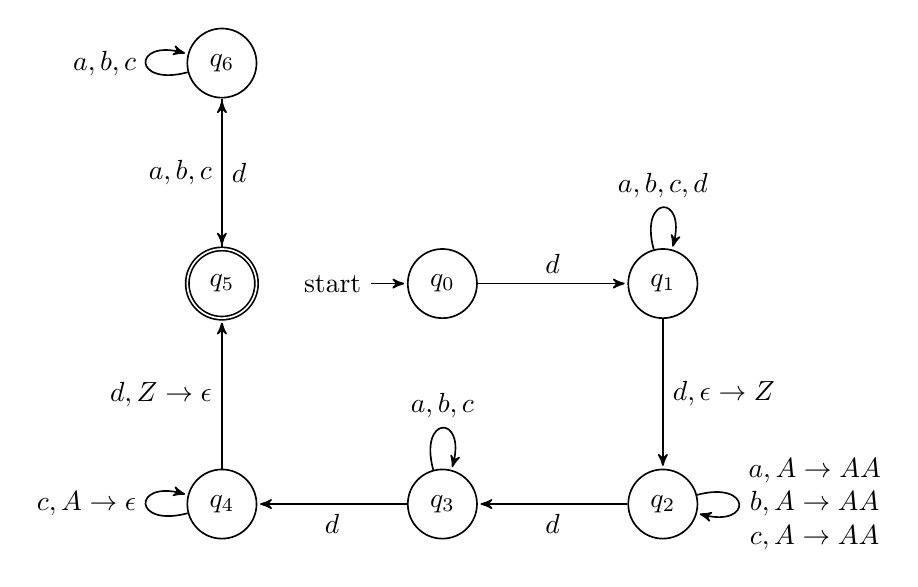
\begin{tikzpicture}[->,>=stealth',shorten >=1pt,auto,node distance=2.8cm,
                    semithick]

  \node[initial,state]   (A)              {$q_0$};
  \node[state]           (B) [right of=A] {$q_1$};
  \node[state]           (C) [below of=B] {$q_2$};
  \node[state]           (D) [left of=C]  {$q_3$};
  \node[state]           (E) [left of=D]  {$q_4$};
  \node[state,accepting] (F) [left of=A]  {$q_5$};
  \node[state]           (G) [above of=F] {$q_6$};

  \path (A) edge              node {$d$}                 (B)
        (B) edge [loop above] node {$a,b,c,d$}           (B)
            edge              node {$d, \epsilon \to Z$} (C)
        (C) edge [loop right, align=center] node {
                                   $a, A \to AA$ \\
                                   $b, A \to AA$ \\
                                   $c, A \to AA$}         (C)
            edge              node {$d$}                 (D)
        (D) edge [loop above] node {$a,b,c$}             (D)
            edge              node {$d$}                 (E)
        (E) edge [loop left]  node {$c, A \to \epsilon$} (E)
            edge              node {$d, Z \to \epsilon$} (F)
        (F) edge              node {$a,b,c$}             (G)
        (G) edge [loop left]  node {$a,b,c$}             (G)
            edge              node {$d$}                 (F);
\end{tikzpicture}

\emph{(Whenever stack symbols neither read, nor added nor removed, they are}
\emph{omitted from the diagram to make it easier to read)}

The rationale for this diagram is as follows:
\begin{enumerate}
\item Read the first $d$.
\item Keep reading as many of $as$, $bs$, $cs$ or $ds$ as necessary.
\item Non-deterministically, upon reading $d$ assume reading the
``special'' sequence of $as$, $bs$ and $cs$, which must be equal
in length to the sequence of $cs$ to follow after.
``Notice'' this event by pushing $Z$ on stack.
\item Read $as$, $bs$ and $cs$ pushing $As$ on stack.
\item Read $d$.
\item Read any number of $as$, $bs$ or $cs$.
\item Upon reading $d$ start reading $cs$ while discarding $As$.
\item Once you pop $Z$ you also must read $d$, this will ensure the number of
$cs$ is the same as the number of $as$, $bs$ and $cs$, read in step (4).
\item After this had happened, we've already found the ``special'' substring,
now we just need to make sure to terminate when we read $d$.
\end{enumerate}

\subsection{Problem 5}
\label{sec-1-5}
Given language $L=\{a^kb^ic^jd^{j-i}e^k \;|\; 1 \leq i \leq j, k \geq 2 \}$
build a deterministic PDA accepting it.

\subsubsection{Answer 7}
\label{sec-1-5-1}
First, to better understand the language, I'll give its grammar:

\begin{align*}
  &S \to aaXbb \\
  &X \to aXb \;|\; YZ \\
  &Y \to bYc \;|\; bc \\
  &Z \to cZd \;|\; \epsilon \;.
\end{align*}

Informally, the language consists of three ``major chunks'':
\begin{enumerate}
\item An even number of $as$ and $es$ on the edges (which also, eventually,
must be greater than four).
\item The middle ``chunk'' is split into two parts:
\begin{itemize}
\item An even number of $bs$ and $cs$, necessarily more than two characters
long.
\item Followed by the optional third ``chunk'' of an even number of $cs$ and
$ds$.
\end{itemize}
\end{enumerate}


Having realized this, we are now equipped to build an automaton:

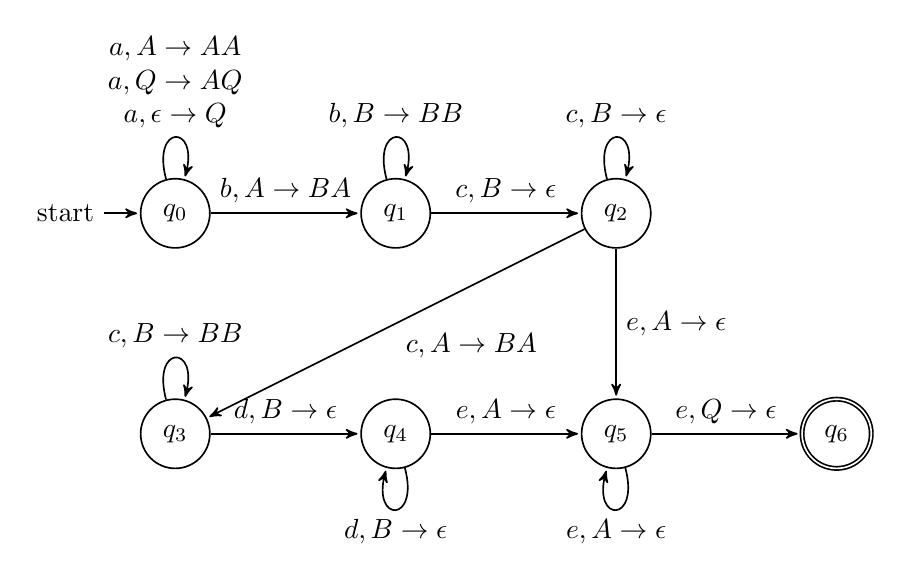
\begin{tikzpicture}[->,>=stealth',shorten >=1pt,auto,node distance=2.8cm,
                    semithick]

  \node[initial,state]   (A)              {$q_0$};
  \node[state]           (B) [right of=A] {$q_1$};
  \node[state]           (C) [right of=B] {$q_2$};
  \node[state]           (D) [below of=A] {$q_3$};
  \node[state]           (E) [right of=D] {$q_4$};
  \node[state]           (F) [right of=E] {$q_5$};
  \node[state,accepting] (G) [right of=F] {$q_6$};

  \path (A) edge [loop above, align=center] node {
                                    $a, A \to AA$ \\
                                    $a, Q \to AQ$ \\
                                    $a, \epsilon \to Q$} (A)
            edge              node {$b, A \to BA$}       (B)
        (B) edge [loop above] node {$b, B \to BB$}       (B)
            edge              node {$c, B \to \epsilon$} (C)
        (C) edge [loop above] node {$c, B \to \epsilon$} (C)
            edge              node {$c, A \to BA$}       (D)
            edge              node {$e, A \to \epsilon$} (F)
        (D) edge [loop above] node {$c, B \to BB$}       (D)
            edge              node {$d, B \to \epsilon$} (E)
        (E) edge [loop below] node {$d, B \to \epsilon$} (E)
            edge              node {$e, A \to \epsilon$} (F)
        (F) edge [loop below] node {$e, A \to \epsilon$} (F)
            edge              node {$e, Q \to \epsilon$} (G);
\end{tikzpicture}

In words, this automaton can be described as:
\begin{enumerate}
\item Read an $a$ and put $Q$ on stack.
\item Read another $a$ and put $A$ on stack (this is to satisfy $\abs{a^k} \geq
       2$.)
\item Keep reading $as$.  While you read $as$ push $A$ on the stack.
\item Once you read $b$, start pushing $Bs$ on the stack.
\item Once you read $c$, start popping $Bs$ from the stack.
\item Once no $Bs$ remain on the stack, if you read $c$, this means
$j > i$, keep reading $cs$ while pushing $Bs$ on the stack.
\begin{itemize}
\item When you encounter $d$, you need to stard popping $Bs$ from the stack.
\item Once you read $d$, but you see $A$ on the stack, move to (8).
\end{itemize}
\item Otherwise, $i = j$, hence you must be reading $d$.  Skip to
the next state.
\item Now you must be reading $e$.  Keep reading $es$ as long as there
are $As$ on the stack.
\item Once you encounter $Q$ on the stack, this is also the final $e$.
If the input ends here, you are done!
\end{enumerate}
\subsection{Problem 6}
\label{sec-1-6}
Given PDA $M$ accepting language $L$ by reaching an accepting state,
construct PDA $N$, accepting language $L^*$.

\subsubsection{Answer 8}
\label{sec-1-6-1}
Informally, all we need to do is to add transitions between the accepting
states and the initial state of $M$ to get $N$.  There is a caveat: if we
accept by reaching certain state, there might be symbols on the stack that
will affect the way the automaton is restarded.  To take care of these
``leftovers'', I suggest adding an extra state, which reads no input, and
discards all stack symbols until it sees the initial stack symbol.  Once it
sees it, the automaton can restart.

More formally, let $M=\langle Q, \Sigma, \Gamma, \delta, q_0, Z, F \rangle$,
where $Q$ is the finite set of states, $\Sigma$ is the input alphabet,
$\Gamma$ is the stack alphabet, $\delta$ is the relation $Q \times (\Sigma
    \cup \{ \epsilon \}) \times \Gamma \times Q \times \Gamma^*$ defining
transitions of $M$.  $q_0$ is the initial state, $Z$ is the initial stack
symbol, $F \subset Q$ is the set of all accepting states.

Then, $N=\langle Q_n, \Sigma, \Gamma, \delta_n, q_0, Z, F \rangle$, where
$Q_n = Q \cup \{q_n\}$, $q_n$ been a state I will describe shortly.

\begin{align*}
  \delta_n = \delta \cup
  \{&(q_n, \epsilon, \gamma \in \Gamma \setminus \{Z\}, q_n, \epsilon), \\
    &(q_n, \epsilon, Z, q_0, Z), \\
    &(q_f \in F, \epsilon, \gamma \in \Gamma \setminus \{Z\}, q_n, \epsilon), \\
    &(q_f \in F, \epsilon, Z, q_0, Z)\}
\end{align*}


reading as: when in state $q_n$ reading no input, $N$ sees $\gamma$ on stack
it must pop $\gamma$ from stack and remain in $q_n$, otherwise, if it reads
$Z$ symbol on stack, it must transition to $q_0$, leaving the initial stack
symbol unchanged.  On top of it, for every accepting state $q_f$, there is a
transition on any symbol, except the initial stack symbol to $q_n$.
Finally, if the accepting state $q_f$ already reads the initial stack symbol
$Z$, it must tranzition to initial state $q_0$.
% Emacs 24.5.1 (Org mode 8.2.10)
\end{document}
